\documentclass[a4paper,french]{paper}
\usepackage{../../_latex_assets/villemejane_iogs_ceti}

%Informations about this document 
%------------------------------------------
\def\module{Conception Electronique pour le Traitement de l'Information}
\def\moduleAbrege{5N-027-SCI / CéTI}
\def\annee{}

\def\titre{Bloc 4 / Systèmes et asservissement}
\author{Julien VILLEMEJANE}

\subtitle{Bloc4}
\institution{LEnsE / Institut d'Optique Graduate School}

\title{\titre}
\begin{document} 
%Beginning First Page. 
%------------------------------------------
\enteteThematiqueObligatoire{}

%Beginning Content. 
%------------------------------------------

\textbf{Objectifs}

Ce bloc de TD va vous permettre de découvrir un autre outil de calcul numérique, \textbf{MatLab} et son extension graphique \textbf{SimuLink} dans le cadre de l'\textbf{analyse de systèmes} pouvant se mettre sous forme d'une fonction de transfert.

\textbf{Ressources}

Tutoriels disponibles à l'adresse suivante :  http://lense.institutoptique.fr/matlab/ 

\bigskip

%%%%%%%%%%%%%%%%%%%
\encadreTDExo{4.1 - Modéliser et simuler un système du premier ordre}{
De manière graphique, à l'aide de \textbf{Simulink}, on souhaite simuler la \textbf{réponse à un échelon} du système dont la fonction de transfert est la suivante :

$$H(j\omega) = \frac{H_0}{1 + j \cdot \frac{\omega}{\omega_0}}$$

avec $H_0 = 5$ et $\omega_0 = 500\operatorname{rd/s}$.

\medskip

A l'aide du tutoriel \textbf{Matlab} / \textsc{Systèmes et asservissement / Approche graphique / SimuLink}, vous devriez aboutir à un schéma de ce type,  :

\begin{center}
	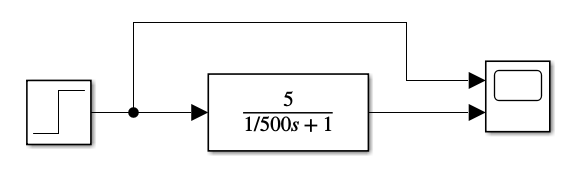
\includegraphics[width=8cm]{images/simulink_sys_1.png}
\end{center}
 
}


\encadreTDExo{4.2 - Modéliser et simuler un système du premier ordre rebouclé}{
De manière graphique, à l'aide de \textbf{Simulink}, on souhaite simuler la \textbf{réponse à un échelon} du modèle du premier ordre d'un Amplificateur Linéaire Intégré (ALI) en \textbf{boucle ouverte} puis en mode \textbf{suiveur}.

On prendra un ALI dont les paramètres sont les suivants : $A_0 = 10^5$ et $GBP = 3~\operatorname{MHz}$.
 
}

\encadreTDExo{4.3 - Asservir un système et instabilité}{
De manière graphique, à l'aide de \textbf{Simulink}, on souhaite simuler la \textbf{réponse à un échelon} puis la \textbf{réponse en fréquence} du système donné par la fonction de transfert suivante : 

$$H(j\omega) = \frac{H_0}{H_0 + (1 + \frac{j \cdot \omega}{\omega_0})^3}$$

pour $\omega_0 = 1000\operatorname{rd/s}$ et $H_0 = 1$, puis $H_0 = 10$ et $H_0 = 50$.

Vous pouvez vous inspirer du tutoriel \textbf{Matlab} / \textsc{Systèmes et réponse en fréquence / Approche graphique / SimuLink}.
}

\encadreTDExo{4.4 - Modéliser et simuler un système asservi du second ordre}{
De manière graphique, à l'aide de \textbf{Simulink}, on souhaite simuler la \textbf{réponse à un échelon} puis la \textbf{réponse en fréquence} du modèle d'un montage transimpédance.

\begin{center}
	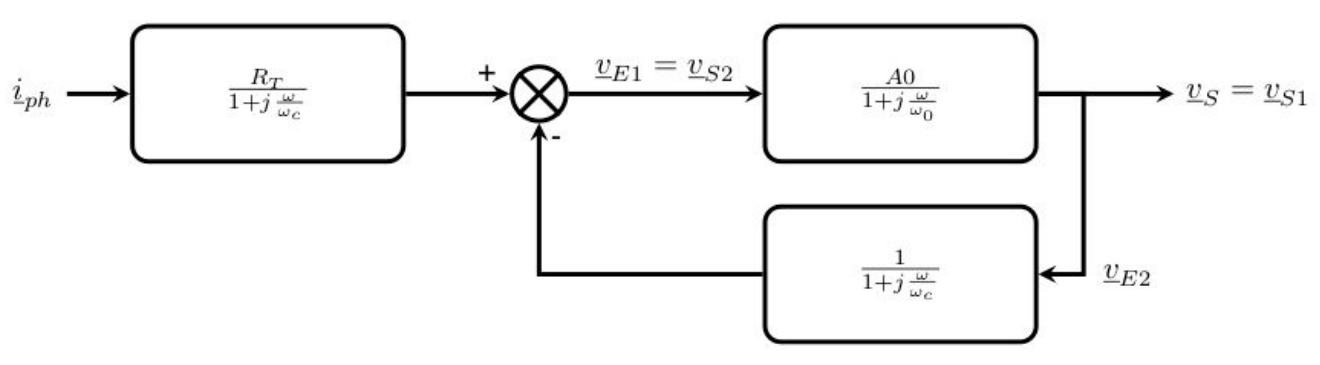
\includegraphics[width=15cm]{images/transimpedance_modele.png}
\end{center}

On prendra un ALI dont les paramètres sont les suivants : $A_0 = 10^5$ et $GBP = 3~\operatorname{MHz}$.

On prendra une photodiode dont la capacité vaut $C_0 = 50\operatorname{pF}$ et une résistance de contre-réaction $R_{PHD} = 100\operatorname{k\Omega}$.
 
}


\encadreTDExo{4.5 - Simuler un système - Approche non graphique}{
A l'aide de \textbf{Matlab}, on souhaite simuler la \textbf{réponse à un échelon} puis la \textbf{réponse en fréquence} du système donné par la fonction de transfert suivante : 

$$H(j\omega) = \frac{1}{1 + 2 \cdot m \cdot \frac{j \cdot \omega}{\omega_0} + (\frac{j \cdot \omega}{\omega_0})^2}$$

avec $m = 0.3$ et $\omega_0 = 800\operatorname{rd/s}$

On souhaite également montrer l'impact du choix du facteur $m$ (facteur d'amortissement) sur la réponse impulsionnelle du système.

\bigskip

Vous pouvez vous inspirer du tutoriel \textbf{Matlab} / \textsc{Systèmes et asservissement / Approche Système}.
}

\encadreTDExo{4.6 - Asservir un système - Approche non graphique}{
A l'aide de \textbf{Matlab}, on souhaite simuler la \textbf{réponse à un échelon} puis la \textbf{réponse en fréquence} du système précédent rebouclé à l'aide d'un gain de facteur $K = \frac{1}{20}$.
}

\encadreTDExo{4.7 - Définir les marges de sécurité d'un système}{
A l'aide de \textbf{Matlab}, on souhaite identifier les marges de sécurité en terme de phase et de gain du système suivant :

$$H(j\omega) = \frac{H_0}{H_0 + (1 + \frac{j \cdot \omega}{\omega_0})^3}$$

pour $\omega_0 = 1000\operatorname{rd/s}$ et $H_0 = 1$, puis $H_0 = 10$ et $H_0 = 50$.

On souhaite également corriger ce système avec un correcteur proportionnel et vérifier la limite de stabilité.

\bigskip

Vous pouvez vous inspirer du tutoriel \textbf{Matlab} / \textsc{Systèmes et asservissement / Approche Système}.
}


%\includepdf[pages=-]{doc/MAX296.pdf}

\end {document}